\subsection{Buscar una ley en el portal de edición}

\begin{figure}[H]
\centerline{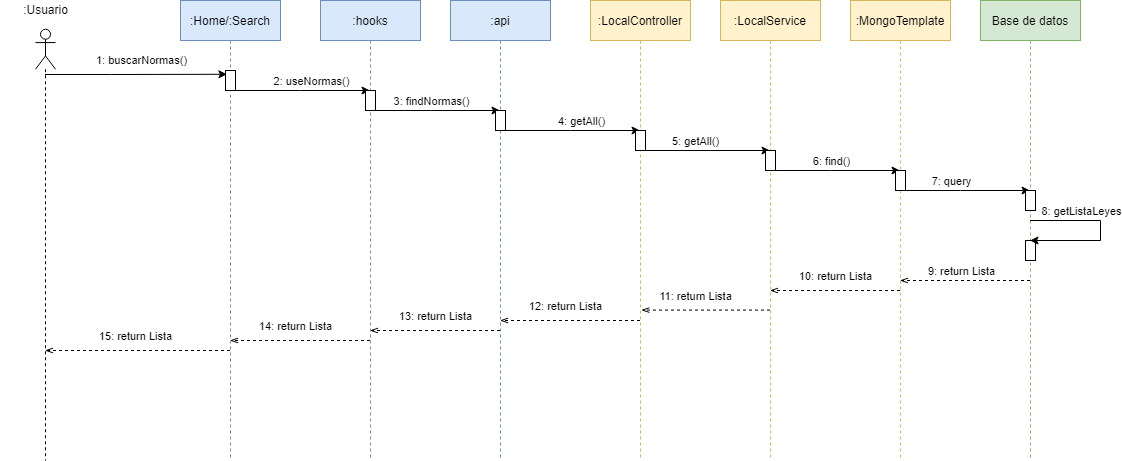
\includegraphics[width=15cm]{figuras/diseño/BuscarLeyLEXGAL.png}}
\caption{Diagrama de secuencia de la búsqueda de una ley en la aplicación.}
\label{enlaceDBuscarLEXGALCuerpo}
\end{figure}

En la \hyperref[enlaceDBuscarLEXGALCuerpo]{Figura 3.11} se representa la operación de búsqueda de leyes en la base de datos de la aplicación. En este caso, puede ser que se encuentren o no leyes, devolviendo las encontradas en el primero de los casos. Esta operación se puede realizar desde las páginas {\bf Home} y {\bf Search} del cliente. Se puede resumir en los siguientes pasos:

\begin{enumerate}
    \item El usuario pincha en buscar leyes en la página de búsqueda, con el texto de sumario si este ha escrito algo, o sin él.
    \item Este método invoca al hook {\it useNormas()} del archivo contenido en {\bf hooks}.
    \item Se invoca al método {\it findNormas()} de la carpeta {\bf api}.
    \item Se hace un llamamiento mediante una solicitud HTTP al servidor. En concreto, a la función {\it getAll()} de {\bf LocalController}, pues se hace un GET. Se comprueba en los filtros que el usuario está autenticado.
    \item Se llama al servicio {\it getAll()} de {\bf FinalDocumentService}.
    \item Se invoca la operación {\it find()} de {\bf MongoTemplate}, pues se busca según un texto, páginas y también tamaño de búsqueda.
    \item Se invoca la operación de recuperar en la base de datos de MongoDB.
    \item Se recuperan las leyes encontradas en la base de datos.
    \item Se procede a devolver la respuesta al usuario desde este paso, realizando el proceso inverso. El usuario recibirá las leyes encontradas de forma paginada, según el texto de sumario que había escrito.
\end{enumerate}